\documentclass[lettersize,onecolumn]{IEEEtran}
\usepackage{amsmath,amsfonts}
\usepackage{algorithmic}
\usepackage{algorithm}
\usepackage{array}
\usepackage[caption=false,font=normalsize,labelfont=sf,textfont=sf]{subfig}
\usepackage{textcomp}
\usepackage{stfloats}
\usepackage{url}
\usepackage{verbatim}
\usepackage{graphicx}
\usepackage{cite}
\usepackage{booktabs}
\usepackage{multirow}
\usepackage{caption}
\usepackage{tabularx}
\hyphenation{op-tical net-works semi-conduc-tor IEEE-Xplore}
% updated with editorial comments 8/9/2021

\begin{document}
	
	\title{An Improved Differential Evolution-Based Hand-Eye Calibration Optimization Algorithm with Elastic Net Regularization: Supplementary File}
	
	\author{Anonymous~\IEEEmembership{}\\
		\vspace{0.3cm}
		\normalsize This is the supplementary material for the paper. It contains extra tables and figures concerning the model structure and experimental results.
		% <-this % stops a space
		\thanks{}}% <-this % stops a space
	
	% The paper headers
	\markboth{}%
	{Shell \MakeLowercase{\textit{et al.}}: A Sample Article Using IEEEtran.cls for IEEE Journals}
	
	\IEEEpubid{}
	% Remember, if you use this you must call \IEEEpubidadjcol in the second
	% column for its text to clear the IEEEpubid mark.
	
	\maketitle
	\IEEEpubidadjcol
	
	\section{Additional Tables}
	\renewcommand{\thetable}{S.I}
\begin{table*}[!htb]
	\caption{Joint angles of the industrial robot movement}
	\label{tab1}
	\centering
	\footnotesize
	\begin{tabular*}{\textwidth}{@{\extracolsep{\fill}}c cccccc|c cccccc}
		\toprule
		No. & \(q_1\) & \(q_2\) & \(q_3\) & \(q_4\) & \(q_5\) & \(q_6\) & No. & \(q_1\) & \(q_2\) & \(q_3\) & \(q_4\) & \(q_5\) & \(q_6\) \\
		\midrule
		1  & -10.52 & -8.05 & -6.52 & -1.60 & 89.55 & -4.10 & 21 & -11.40 & -11.88 & -6.52 & -5.72 & 92.79 & -4.10 \\
		2  & -16.48 & -8.05 & -6.52 & -1.60 & 89.55 & -4.10 & 22 & -11.40 & -11.88 & -6.52 & -5.72 & 88.61 & -4.10 \\
		3  & -13.21 & -7.52 & -6.52 & -1.60 & 89.55 & -4.10 & 23 & -11.40 & -11.88 & -6.52 & -7.77 & 88.61 & -4.10 \\
		4  & -8.24  & -7.52 & -6.52 & -1.60 & 89.55 & -4.10 & 24 & -11.40 & -11.88 & -6.52 & 2.35  & 88.61 & -4.10 \\
		5  & -5.32  & -7.52 & -6.52 & -1.60 & 89.55 & -4.10 & 25 & -11.40 & -11.88 & -6.52 & 2.35  & 87.42 & -4.10 \\
		6  & -4.20  & -7.62 & -6.52 & -1.60 & 89.55 & -4.10 & 26 & -11.40 & -11.88 & -6.52 & 2.35  & 92.60 & -4.10 \\
		7  & -3.88  & -9.90 & -6.52 & -1.60 & 89.55 & -4.10 & 27 & -11.40 & -11.88 & -6.52 & 4.17  & 92.60 & -4.10 \\
		8  & -10.18 & -9.90 & -6.52 & -1.60 & 89.55 & -4.10 & 28 & -11.40 & -11.88 & -6.52 & 4.17  & 93.63 & -4.10 \\
		9  & -13.68 & -9.90 & -6.52 & -1.60 & 89.55 & -4.10 & 29 & -11.40 & -11.88 & -6.52 & 4.17  & 89.49 & -4.10 \\
		10 & -16.51 & -11.88 & -6.52 & -1.60 & 89.55 & -4.10 & 30 & -11.40 & -11.88 & -6.52 & -1.48 & 89.49 & -4.10 \\
		11 & -11.40 & -11.88 & -6.52 & -1.60 & 89.55 & -4.10 & 31 & -11.40 & -11.88 & -6.52 & -1.48 & 93.91 & -4.10 \\
		12 & -11.40 & -11.88 & -6.52 & -1.60 & 93.12 & -4.10 & 32 & -11.40 & -11.88 & -6.52 & -6.45 & 93.79 & -4.10 \\
		13 & -11.40 & -11.88 & -6.52 & 2.79  & 93.12 & -4.10 & 33 & -11.40 & -11.88 & -6.52 & -6.45 & 88.66 & -4.10 \\
		14 & -11.40 & -11.88 & -6.52 & -4.13 & 93.12 & -4.10 & 34 & -11.40 & -11.88 & -6.52 & 2.34  & 88.66 & -4.10 \\
		15 & -11.40 & -11.88 & -6.52 & -4.13 & 88.56 & -4.10 & 35 & -11.40 & -11.88 & -6.52 & 2.34  & 94.15 & -4.10 \\
		16 & -11.40 & -11.88 & -6.52 & -6.95 & 88.56 & -4.10 & 36 & -11.40 & -11.88 & -6.52 & 4.69  & 93.65 & -4.10 \\
		17 & -11.40 & -11.88 & -6.52 & 1.67  & 88.56 & -4.10 & 37 & -16.25 & -11.43 & -6.52 & 4.69  & 93.65 & -4.10 \\
		18 & -11.40 & -11.88 & -6.52 & 1.67  & 92.98 & -4.10 & 38 & -18.82 & -11.43 & -6.52 & 4.69  & 93.65 & -4.10 \\
		19 & -11.40 & -11.88 & -6.52 & 4.23  & 92.98 & -4.10 & 39 & -22.21 & -11.45 & -6.52 & 4.69  & 93.65 & -4.10 \\
		20 & -11.40 & -11.88 & -6.52 & -0.19 & 92.98 & -4.10 & 40 & -24.75 & -11.58 & -6.52 & 4.69  & 93.65 & -4.10 \\
		\bottomrule
	\end{tabular*}
\end{table*}
	
	\renewcommand{\thetable}{S.II}
\begin{table*}[!htb]
	\caption{Algorithm Parameter Settings}
	\label{tab2}
	\centering
	\footnotesize
	\begin{tabular*}{\textwidth}{@{\extracolsep{\fill}}m{0.12\textwidth}p{0.78\textwidth}}
		\toprule
		Algorithm & Parameter Settings \\
		\midrule
		IDER & \(N_P = 100\); \(T = 120\); Scaling factor \(F = 0.6\); Crossover rate \(CR = 0.9\). \\
		PSO  & \(N_P = 100\); \(T = 120\); Inertia weight \(\omega = 0.6\); Learning factors \(c_1 = 1.2\), \(c_2 = 1.2\). \\
		DE   & \(N_P = 100\); \(T = 120\); Scaling factor \(F = 0.6\); Crossover rate \(CR = 0.9\). \\
		GA   & \(N_P = 100\); \(T = 120\); Crossover rate: 0.9; Mutation rate: 0.08; Tournament selection size: 3. \\
		QPSO & \(N_P = 100\); \(T = 120\); Contraction-expansion coefficient: 1; Mean optimal coefficient: 0.06. \\
		CS   & \(N_P = 100\); \(T = 120\); Abandonment probability \(pa = 0.15\); Step size scaling factor: 0.6; Characteristic exponent \(\beta = 1.8\). \\
		GWO  & \(N_P = 100\); \(T = 120\); Initial convergence factor: 1.8; Final convergence factor: 0. \\
		SCA  & \(N_P = 100\); \(T = 120\); Initial attenuation factor: 5; Final attenuation factor: 0. \\
		ABC  & \(N_P = 100\); \(T = 120\); Limit: 15; Scout bee trigger frequency: 12. \\
		FA   & \(N_P = 100\); \(T = 120\); Maximum attractiveness: 1; Light absorption coefficient: 0.8; Random step factor: 0.7. \\
		\bottomrule
	\end{tabular*}
\end{table*}

	
\onecolumn

\clearpage

	\section{Additional Figures}
	
	\renewcommand{\thefigure}{S.\arabic{figure}}
	\begin{figure}[!htb]
		\centering
		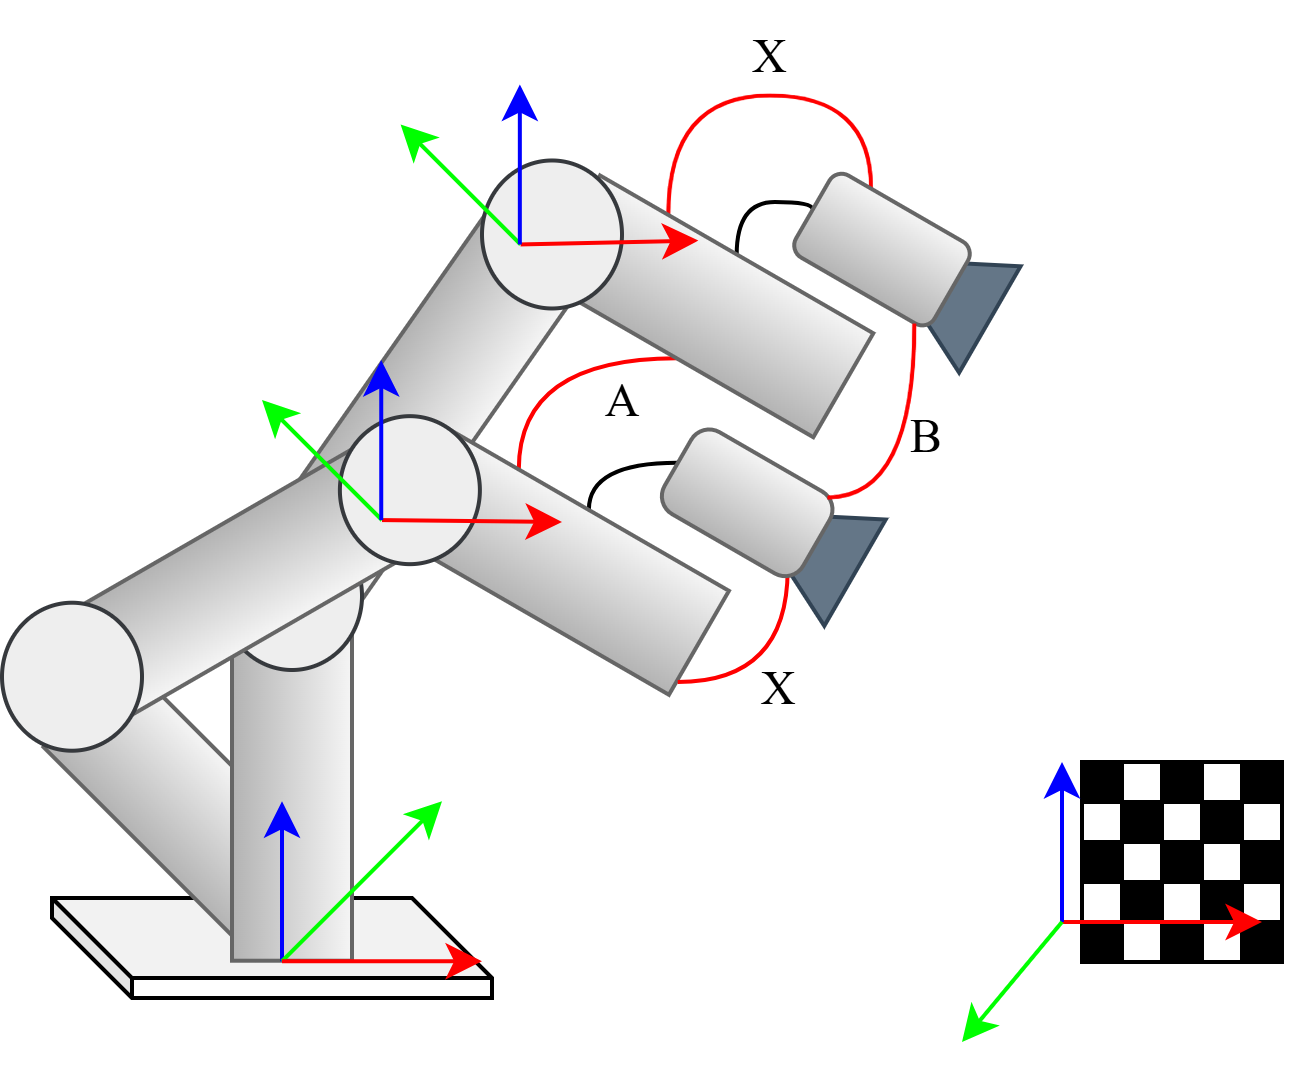
\includegraphics[width=4.5in]{S1}
		\caption{Formulating the AX=XB problem.}
		\label{figS1}
	\end{figure}
	
	\begin{figure}[!htb]
		\centering
		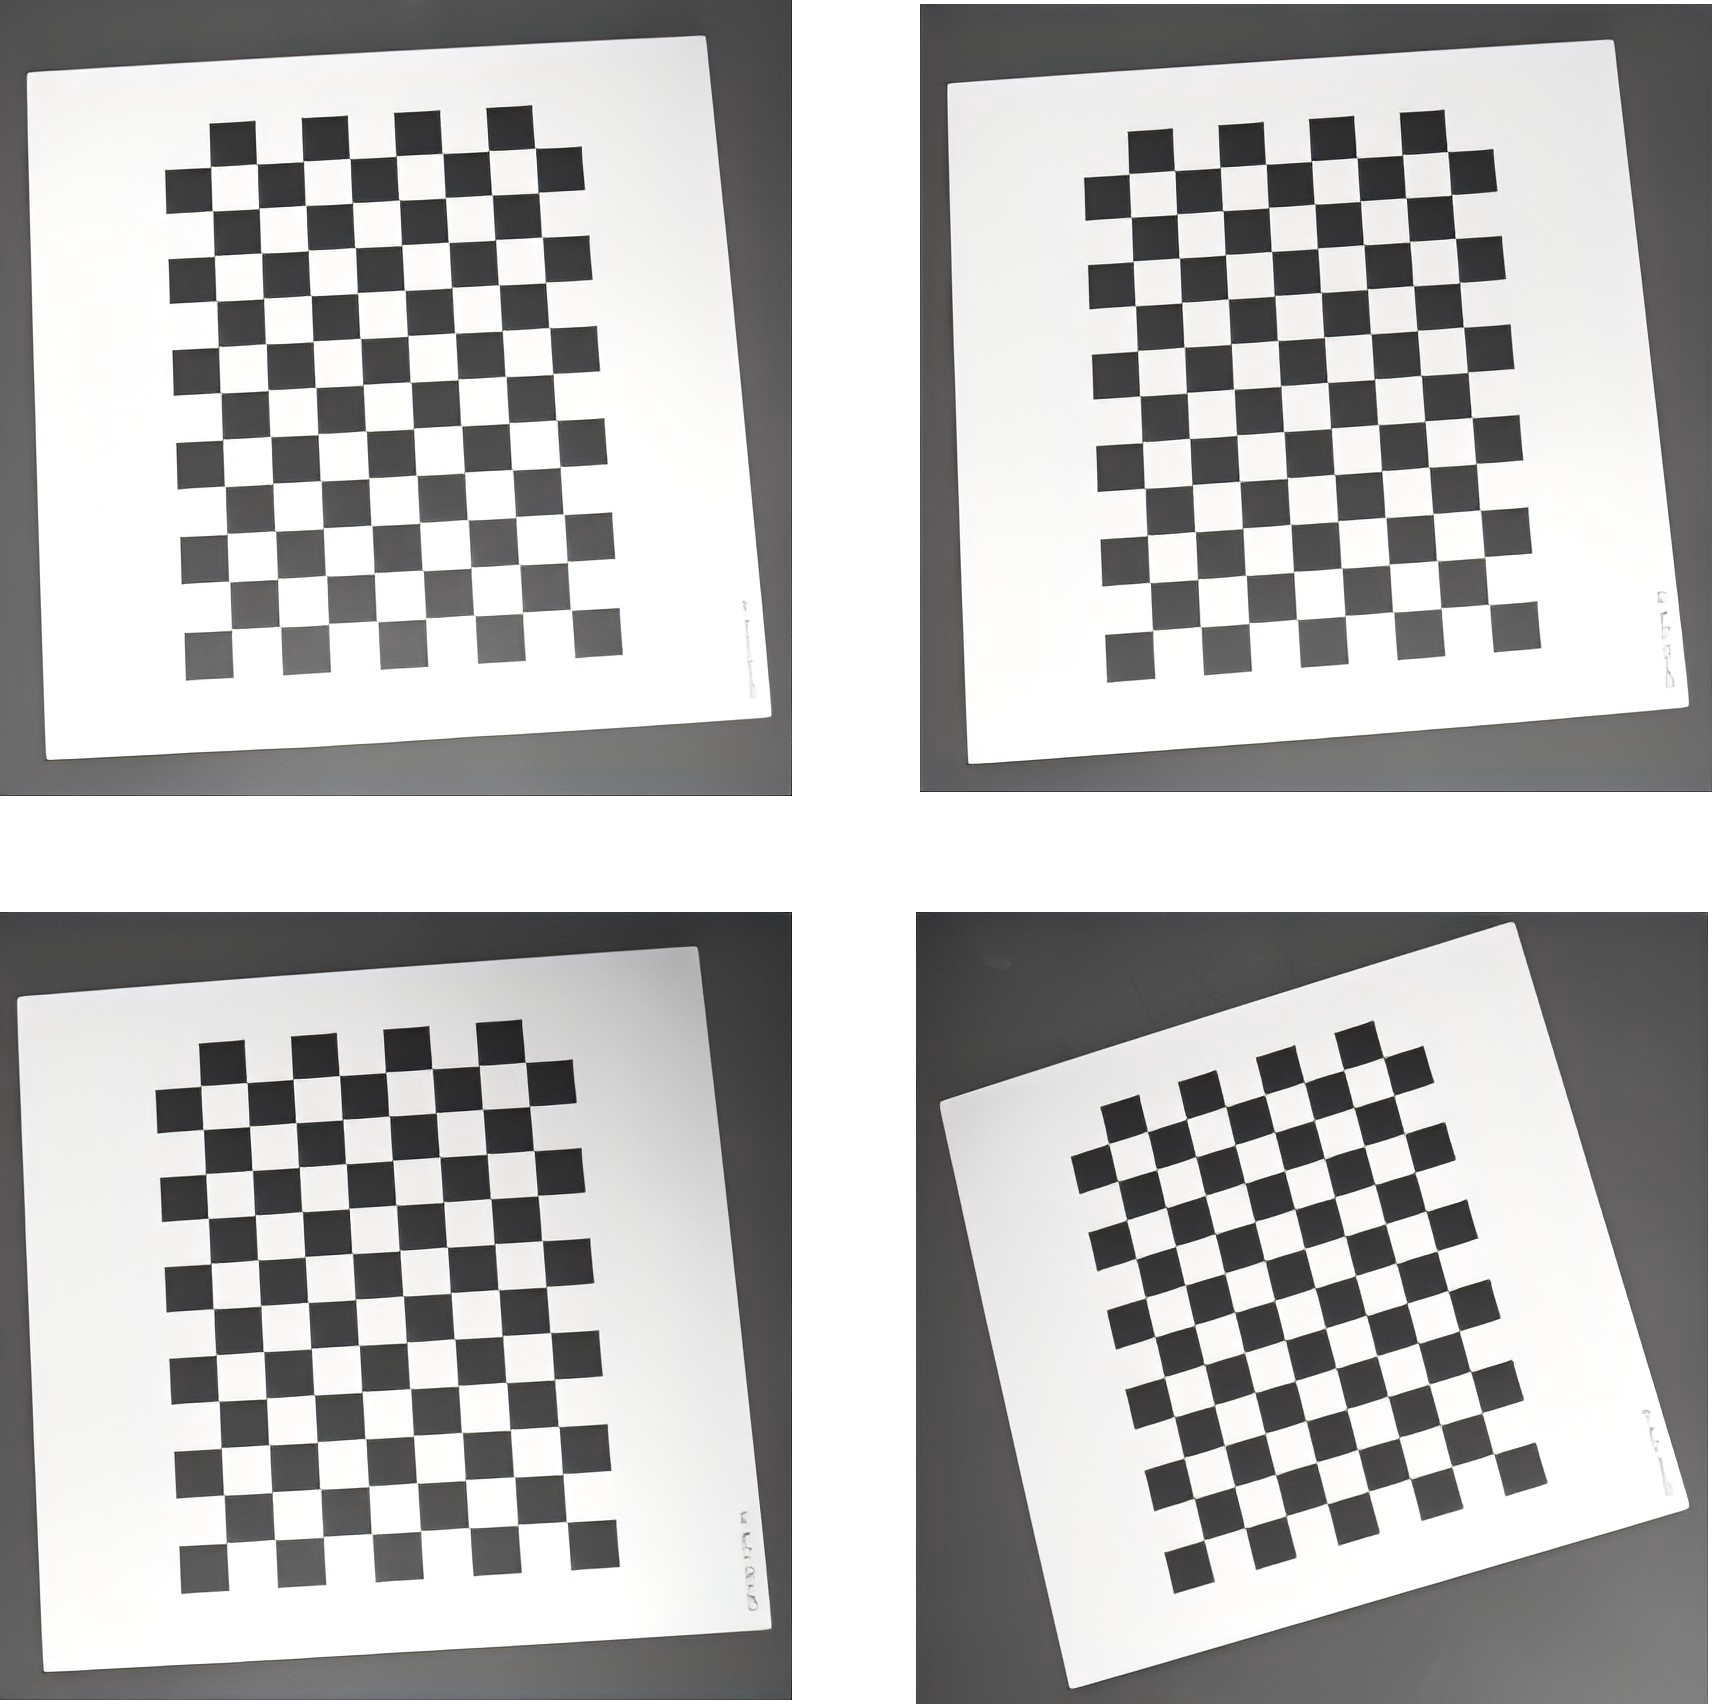
\includegraphics[width=4.5in]{S2}
		\caption{Images of the calibration board captured from different poses.}
		\label{figS2}
	\end{figure}
	
\end{document}


